\documentclass[11pt]{article}
\usepackage[margin=1in]{geometry}
\usepackage[T1]{fontenc}
\usepackage{lmodern}
\usepackage{amsmath,amssymb}
\usepackage{booktabs}
\usepackage{siunitx}
\usepackage{graphicx}
\usepackage{xcolor}
\usepackage{ifthen}
\usepackage[numbers,sort&compress]{natbib}
\usepackage{hyperref}
\usepackage{cleveref}
\hypersetup{colorlinks=true,linkcolor=blue!50!black,citecolor=blue!50!black,urlcolor=blue!50!black}

% GENERATED by figures/make_figures.py from results/rtx3070-laptop.json -- do not edit by hand.
\newcommand{\benchProvisional}{false}
\newcommand{\benchMode}{full}
\newcommand{\benchFile}{rtx3070-laptop.json}
\newcommand{\gpuName}{NVIDIA GeForce RTX 3070 Laptop GPU}
\newcommand{\copyBW}{360.9}
\newcommand{\specBW}{448}
\newcommand{\philoxRate}{112.6}
\newcommand{\callsPerWord}{3.80}
\newcommand{\bitsPerSpin}{7.6}
\newcommand{\memCeilInt}{120}
\newcommand{\memCeilMsc}{962}
\newcommand{\rngCeilInt}{450}
\newcommand{\rngCeilMsc}{1894}
\newcommand{\callsPerWordWarp}{6.30}
\newcommand{\bitsPerSpinWarp}{12.6}
\newcommand{\rngCeilMscWarp}{1144}
\newcommand{\bestFlips}{419.3}
\newcommand{\bestBackend}{CUDA C (CuPy) (msc)}
\newcommand{\bestL}{4096}
\newcommand{\bestPctCopy}{43.6}
\newcommand{\bestPctSpec}{35.1}
\newcommand{\bestGBs}{157.2}
\newcommand{\bestPyFlips}{371.9}
\newcommand{\bestPyBackend}{Warp (msc)}
\newcommand{\bestPyPctCopy}{38.6}
\newcommand{\bestIntFlips}{80.8}
\newcommand{\bestIntBackend}{CUDA C (CuPy)}
\newcommand{\bestIntPctCopy}{67.2}
\newcommand{\numpyFlips}{0.049}
\newcommand{\speedupVsNumpy}{8558}
\newcommand{\nRuns}{98}
\newcommand{\maxSpins}{1.72\times 10^{10}}
\newcommand{\ablEager}{211.8}
\newcommand{\ablLazy}{419.3}
\newcommand{\ablPerSite}{49.9}
\newcommand{\ablCudaInt}{80.8}
\newcommand{\dslIntBackend}{Triton}
\newcommand{\dslIntPctCuda}{72}
\newcommand{\dslMscBackend}{Warp}
\newcommand{\dslMscPctCuda}{89}
\newcommand{\bestPctRngWarp}{36.7}
\newcommand{\valQuick}{false}
\newcommand{\valIdentical}{all}
\newcommand{\valNIdentity}{33}
\newcommand{\valEmaxErr}{4.3\times 10^{-3}}
\newcommand{\valEmaxZ}{3.29}
\newcommand{\valMmaxErr}{3.8\times 10^{-4}}
\newcommand{\valTcTwo}{2.2712}
\newcommand{\valTcTwoErr}{0.09}
\newcommand{\valTcThree}{4.5102}
\newcommand{\valTcThreeErr}{0.03}
\newcommand{\valThreeZ}{1.19}
\newcommand{\valLtwo}{128}
\newcommand{\valLthree}{32}
\newcommand{\perfTable}{\begin{tabular}{llrrrr}
\toprule
backend & variant & $L$ & flips/ns & GB/s & \% copy \\
\midrule
NumPy & int8 & 1024 & 0.05 & 0.1 & 0.0 \\
torch eager & int8 & 8192 & 0.49 & 1.5 & 0.4 \\
torch.compile & int8 & 8192 & 9.60 & 28.8 & 8.0 \\
Triton & int8 & 2048 & 58.33 & 175.0 & 48.5 \\
Warp & int8 & 2048 & 45.31 & 135.9 & 37.7 \\
Numba-CUDA & int8 & 2048 & 43.64 & 130.9 & 36.3 \\
CUDA C (CuPy) & int8 & 2048 & 80.81 & 242.4 & 67.2 \\
CUDA C (CuPy) & int8-rng-per-site & 4096 & 49.91 & 149.7 & 41.5 \\
NumPy & msc & 1024 & 0.12 & 0.0 & 0.0 \\
Triton & msc & 131072 & 342.43 & 128.4 & 35.6 \\
Warp & msc & 16384 & 371.93 & 139.5 & 38.6 \\
Numba-CUDA & msc & 16384 & 327.36 & 122.8 & 34.0 \\
CUDA C (CuPy) & msc & 4096 & 419.32 & 157.2 & 43.6 \\
CUDA C (CuPy) & msc-eager32 & 4096 & 211.81 & 79.4 & 22.0 \\
\bottomrule
\end{tabular}}
\newcommand{\bestThreeFlips}{77.2}
\newcommand{\bestThreeBackend}{CUDA C (CuPy)}
\newcommand{\bestThreeL}{256}
\newcommand{\bestThreePct}{64.2}
% head-to-head macros from results/counterparts.json
\newcommand{\cpAvailable}{true}
\newcommand{\cpProvisional}{true}
\newcommand{\cpMode}{quick}
\newcommand{\cpCommit}{935796d}
\newcommand{\cpRomeroBasicCudaFlips}{21.4}
\newcommand{\cpRomeroBasicCudaL}{4096}
\newcommand{\cpRomeroBasicPyFlips}{3.0}
\newcommand{\cpRomeroBasicPyL}{4096}
\newcommand{\cpRomeroTensorFlips}{11.1}
\newcommand{\cpRomeroTensorL}{4096}
\newcommand{\cpRomeroOldFlips}{169.2}
\newcommand{\cpRomeroOldL}{4096}
\newcommand{\cpRomeroOptFlips}{201.3}
\newcommand{\cpRomeroOptL}{4096}
\newcommand{\cpOursIntFlips}{63.1}
\newcommand{\cpOursIntL}{4096}
\newcommand{\cpOursIntBackend}{CUDA C (CuPy)}
\newcommand{\cpOursPyIntFlips}{46.9}
\newcommand{\cpOursPyIntL}{4096}
\newcommand{\cpOursPyIntBackend}{Triton}
\newcommand{\cpOursMscFlips}{364.8}
\newcommand{\cpOursMscL}{4096}
\newcommand{\cpOursMscBackend}{CUDA C (CuPy)}
\newcommand{\cpOursPyMscFlips}{300.8}
\newcommand{\cpOursPyMscL}{4096}
\newcommand{\cpOursPyMscBackend}{Warp}
\newcommand{\cpRatioOpt}{1.81}
\newcommand{\cpRatioPyOpt}{1.49}
\newcommand{\cpRatioOld}{2.16}
\newcommand{\cpRatioBasic}{2.95}
\newcommand{\cpRatioPyBasic}{15.49}
\newcommand{\cpOptCompare}{faster than}
\newcommand{\cpPyOptCompare}{faster than}
\newcommand{\cpOldCompare}{faster than}
\newcommand{\cpEnergyL}{4096}
\newcommand{\cpEnergySweeps}{200}
\newcommand{\cpEnergyTheirs}{-1.3826}
\newcommand{\cpEnergyOurs}{-1.3832}
\newcommand{\cpEnergyMaxZ}{0.8}
\newcommand{\cpBasicIdentical}{identical}
\newcommand{\cpPctCopyOpt}{20.9}
\newcommand{\cpPctCopyOld}{70.3}
\newcommand{\cpTable}{\begin{tabular}{llrrrr}
\toprule
code & variant & bits/spin & $L$ & flips/ns & \% copy \\
\midrule
ising-gpu & basic\_cuda & 8 & 4096 & 21.4 & 17.8 \\
ising-gpu & basic\_python & 8 & 4096 & 3.0 & 2.5 \\
ising-gpu & tensorcore & 16 & 4096 & 11.1 & 18.5 \\
ising-gpu & optimized\_old & 4 & 4096 & 169.2 & 70.3 \\
ising-gpu & cuIsingModel & 1 & 4096 & 201.3 & 20.9 \\
\midrule
pyising & Triton (int8) & 8 & 4096 & 46.9 & 39.0 \\
pyising & CUDA C (CuPy) (int8) & 8 & 4096 & 63.1 & 52.5 \\
pyising & Warp (msc) & 1 & 4096 & 300.8 & 31.3 \\
pyising & CUDA C (CuPy) (msc) & 1 & 4096 & 364.8 & 37.9 \\
\bottomrule
\end{tabular}}


\newcommand{\provbanner}{%
  \ifthenelse{\equal{\benchProvisional}{true}}{%
    \begin{center}\fcolorbox{red!70!black}{red!8}{\parbox{0.92\linewidth}{\centering
    \textbf{\textcolor{red!70!black}{PROVISIONAL NUMBERS}}\\[2pt]\small
    Performance numbers come from a development run (\texttt{\benchFile}, mode \texttt{\benchMode})
    on a GPU shared with other jobs. They are not publishable; the final numbers come from
    \texttt{bench/run.py -{}-full} on an idle GPU.}}\end{center}}{}}

\title{Billions of spin flips per second from Python:\\
a roofline study of GPU Ising Monte Carlo}
\author{Walid Hemati\\Independent researcher}
\date{}

\begin{document}
\maketitle
\provbanner

\begin{abstract}
We implement checkerboard Metropolis and heat-bath Monte Carlo for the two- and
three-dimensional Ising model in seven Python-driven backends (NumPy, PyTorch eager,
\texttt{torch.compile}, Triton, NVIDIA Warp, Numba-CUDA and a hand-written CUDA~C reference
compiled at run time through CuPy) and measure every rung of the optimisation ladder against a
roofline built from two measured ceilings: device-to-device copy bandwidth
(\SI{\copyBW}{GB/s}) and the throughput of the Philox4x32-10 counter-based generator
(\SI{\philoxRate}{calls/ns}). All backends share one counter-based random stream, so the
same seed produces bit-identical spin configurations on every backend (\valNIdentity{} of
\valNIdentity{} identity checks pass). With 64 spins per 64-bit word, bit-sliced neighbour
counting, and a \emph{lazy bitwise comparison} that draws on average \bitsPerSpin{} random bits
per spin instead of 32 while sampling the Metropolis acceptance probability exactly, the fastest
variant (\bestBackend) reaches \textbf{\bestFlips{} spin flips per ns} on a single
\gpuName{}, \bestPctCopy\,\% of the measured copy bandwidth under a minimal 0.375-byte-per-update
traffic model. The fastest pure-Python-DSL kernel (\bestPyBackend) reaches \bestPyFlips{}
flips/ns. Measured energies agree with the exact finite-lattice solution (Kaufman,
Ferdinand--Fisher) to within \valEmaxZ{} standard errors at every temperature, magnetisations
with Onsager--Yang, and Binder-cumulant crossings give $T_c$ to \valTcTwoErr\,\% (2D) and
\valTcThreeErr\,\% (3D).
\end{abstract}

\section{Introduction}

The Ising model is the standard benchmark of Monte Carlo simulation on new hardware. Its update
is a handful of integer operations per spin, so on a GPU the cost is set by memory traffic and
by the random number generator, not by floating-point arithmetic. This makes it a clean test
of a broader claim: that Python, used as a host for GPU kernels, can reach the same
\emph{hardware efficiency} as hand-tuned CUDA. We test that claim with a roofline
\citep{Williams2009}: every throughput below is quoted as an absolute rate and as a fraction of a
ceiling measured on the same machine.

Contributions:
\begin{itemize}
  \item An open-source package, \texttt{pyising}, with one common interface over seven backends
        and fourteen backend/variant combinations in 2D and 3D, Metropolis and heat bath, plus a
        Wolff cluster sampler \citep{Wolff1989} for near-critical validation.
  \item A layout-independent Philox4x32-10 \citep{Salmon2011} random stream and integer
        acceptance thresholds, so that the same seed gives bit-identical trajectories on NumPy,
        PyTorch, Triton, Warp, Numba and CUDA~C. The NumPy implementation is the test oracle.
  \item A lazy, lane-parallel bitwise comparison of uniforms against the Metropolis thresholds
        for 1-bit multi-spin coding. It is exact (equivalent to a 32-bit integer comparison)
        and needs on average \callsPerWord{} Philox calls per 64-spin word at $T_c$
        (\callsPerWordWarp{} counting SIMT divergence) instead of 16.
  \item A roofline analysis with two measured ceilings (copy bandwidth and Philox throughput),
        a minimal traffic model for int8 and packed spins, and an honest comparison with
        published GPU Ising codes.
  \item Validation against exact results: the finite-torus energy at all temperatures, the
        spontaneous magnetisation, Binder crossings in 2D and 3D.
\end{itemize}

\section{Background and related work}

\paragraph{Model.} We simulate $H=-J\sum_{\langle ij\rangle}s_is_j$ with $s_i=\pm1$, $J=k_B=1$,
periodic boundaries, on $L\times L$ square and $L^3$ simple-cubic lattices. In 2D the critical
temperature is $T_c=2/\ln(1+\sqrt2)\approx2.269185$ \citep{Onsager1944}, the spontaneous
magnetisation is $m_0=(1-\sinh^{-4}(2/T))^{1/8}$ \citep{Yang1952}, and the free energy of a
finite torus is known in closed form \citep{FerdinandFisher1969}. In 3D the most precise Monte
Carlo estimate is $K_c=J/k_BT_c=0.221\,654\,626(5)$ \citep{Ferrenberg2018}.

\paragraph{Algorithms.} Metropolis \citep{Metropolis1953} and heat-bath updates of one
sublattice of a checkerboard decomposition are independent, which makes them data-parallel.
Near $T_c$ local updates slow down critically; cluster algorithms
\citep{SwendsenWang1987,Wolff1989} avoid this and are used here only for validation. The
Binder cumulant $U_4=1-\langle m^4\rangle/(3\langle m^2\rangle^2)$ \citep{Binder1981} is
size-independent at $T_c$ up to corrections to scaling.

\paragraph{GPU Ising codes.} \citet{Preis2009} ported checkerboard Metropolis to a GeForce
GTX~280 and reported speedups of about 60 (2D) and 35 (3D) over one CPU core.
\citet{Block2010} used multi-spin coding with one bit per spin and reached 7.9 flips/ns on one
Tesla C1060 and 206 flips/ns on 64 such GPUs for an $800\,000^2$ lattice. \citet{Weigel2011}
reported about 0.1\,ns per spin flip in 2D on a Tesla C1060, and \citet{Weigel2012} studied the
performance potential in detail (e.g.\ 0.27\,ns per flip without multi-hit updates on the
C1060). \citet{Yang2019TPU} ran the model on TPU clusters (12.9 flips/ns per TPUv3 core,
5853 flips/ns on 512 cores). \citet{Romero2020} gave the reference implementations for current
NVIDIA hardware: on one Tesla V100-SXM their basic Python version (Numba kernels plus CuPy
random numbers) reaches 43.8 flips/ns, their basic CUDA~C version 67.0 flips/ns, and their
optimised multi-spin-coding version (4 bits per spin, 16 spins per 64-bit word, cuRAND
Philox4\_32\_10 random numbers) 420.8 flips/ns; 16 V100s in a DGX-2H reach 7381 flips/ns. Our
contribution is not a larger aggregate number but the measured efficiency of Python-hosted
kernels against the ceilings of the machine they run on.

\section{Method}

\subsection{Update rules with integer thresholds}
For a site with spin $s$ and neighbour sum $h$, Metropolis flips with probability
$\min(1,e^{-2\beta sh})$ and heat bath sets $s'=+1$ with probability $1/(1+e^{-2\beta h})$.
Both depend only on $X=sh$ (resp.\ $h$) $\in\{-2d,\dots,2d\}$, so we precompute a table of
$2d+1$ unsigned 32-bit thresholds $t_X=\lfloor p_X2^{32}\rfloor$ and accept iff $u<t_X$ for a
uniform 32-bit word $u$. The comparison is exact integer arithmetic, so every backend takes the
same decision for the same $u$; floating-point differences between compilers cannot change a
trajectory.

\subsection{A layout-independent random stream}
Philox4x32-10 \citep{Salmon2011} maps a 128-bit counter and a 64-bit key to four 32-bit words.
Sites of colour $c$ are numbered $n=r\,(L_x/2)+j$ in the compressed checkerboard layout
($r$ the flattened row, $j$ the position among the colour-$c$ sites of the row). Site $n$ in
sweep $t$ uses word $n\bmod4$ of $\mathrm{Philox}(\lfloor n/4\rfloor,t,c,0;\mathrm{seed})$, so
one call serves four sites and the number does not depend on which thread computes it. Our
implementation reproduces the Random123 known-answer vectors.

\subsection{Multi-spin coding with lazy bitwise uniforms}
In the packed variant bit $b$ of word $w$ holds the spin at $j=64w+b$ (1 = up). The
anti-aligned indicators $x_k=s\oplus n_k$ for the four neighbour words (the horizontal one is a
one-bit funnel shift with a carry from the adjacent word) are reduced bit-sliced:
$a_0=\lnot(x_1\lor x_2\lor x_3\lor x_4)$, $a_{\ge2}=(x_1\land x_2)\lor(x_3\land
x_4)\lor((x_1\oplus x_2)\land(x_3\oplus x_4))$ and $a_1=\lnot a_0\land\lnot a_{\ge2}$, where
$a$ is the number of anti-aligned neighbours and $\Delta E=8-4a$. Lanes with $a\ge2$ always flip;
lanes with $a=1$ ($a=0$) flip iff their uniform is below $t_4$ ($t_8$).

Instead of drawing a 32-bit uniform for every lane we build all 64 uniforms at once, most
significant bit first: random word $R_k$ supplies bit $31-k$ of every lane's $u$. With
$T_k$ the lane mask of the threshold bits ($t_4$ on $a_1$ lanes, $t_8$ on $a_0$ lanes) and $D$
the mask of still-undecided lanes,
\begin{equation}
\mathrm{acc}\mathrel{|}=D\land\lnot R_k\land T_k,\qquad D\mathrel{\&}=\lnot(R_k\oplus T_k).
\end{equation}
A lane is decided at the first bit where $u$ and the threshold differ, exactly as in an integer
comparison; if all 32 bits agree, $u=t$ and the move is rejected. The acceptance probability is
therefore exactly $t/2^{32}$, identical to the int8 kernels. The loop stops when $D=0$; each
lane survives a level with probability $1/2$, so a word needs about $\log_2 n+1.3$ levels for
$n$ lanes that need a random decision, and two levels come from one Philox call (128 bits). We
measured \callsPerWord{} Philox calls per word at $T_c$, i.e.\ \bitsPerSpin{} random bits per
spin instead of 32. On SIMT hardware a warp runs the loop until its slowest thread is done; the
per-warp maximum is \callsPerWordWarp{} calls per word (\bitsPerSpinWarp{} bits per spin), still
$2.5\times$ fewer than 16. Since results do not depend on where the loop stops, an eager ablation
that always draws 32 levels produces bit-identical configurations and isolates the cost of
randomness.

\subsection{Measurements and errors}
Energy and magnetisation are reduced on the device (every bond has exactly one colour-0 end,
so $E=-\sum_{i\in0}s_ih_i$; packed lattices use population counts). Errors come from 32-block
binning; Binder errors from a blocked jackknife. Validation runs start from Wolff-equilibrated
configurations, so critical slowing down of the local dynamics affects only the error bars,
not the mean.

\section{Implementation: the optimisation ladder}

\begin{table}[t]
\centering\small
\begin{tabular}{lll}
\toprule
rung & backend & what changes \\
\midrule
0 & NumPy & reference: vectorised Philox on \texttt{uint64}, compressed layout \\
1 & PyTorch eager & same algorithm as tensor ops (dozens of kernels per half sweep) \\
2 & \texttt{torch.compile} & the same Python, fused by Inductor into Triton kernels \\
3 & Triton & hand-written kernel, $[B,4]$ tiles, one Philox call per 4 sites \\
4 & Warp & kernel in Python, 3D launch grid without integer division \\
5 & Numba-CUDA & kernel in Python, compile-time constants by closure \\
6 & CUDA C (CuPy) & \texttt{char4} loads, one thread per 4 sites, NVRTC \\
7 & all GPU DSLs & 1-bit multi-spin coding with lazy bitwise uniforms \\
\bottomrule
\end{tabular}
\caption{Backends and variants. Every row is a registry entry with the same interface; rows 1--6
reproduce rung 0 bit for bit, rung 7 reproduces its own NumPy reference bit for bit.}
\label{tab:ladder}
\end{table}

\Cref{tab:ladder} lists the rungs. All GPU kernels use the compressed checkerboard layout: one
array per colour of shape $(\text{rows},L_x/2)$, so a half sweep reads the opposite colour
array, reads and writes its own, and touches no inactive sites.

\paragraph{Memory-traffic model.} Per half sweep of $N/2$ updates the minimal DRAM traffic is
one read of the own colour, one read of the other colour (neighbours shared through caches) and
one write of the own colour: $3\times$ the spin size per update, i.e.\ \SI{3}{B} for int8 and
\SI{0.375}{B} for 1-bit packing. The copy-bandwidth ceiling is then \memCeilInt{} flips/ns for
int8 and \memCeilMsc{} flips/ns for packed spins. The Philox ceiling is \rngCeilInt{} flips/ns
for one call per four sites and \rngCeilMscWarp{} flips/ns for the lazy packed kernel when the
per-warp number of calls is charged (\rngCeilMsc{} flips/ns with the per-thread mean).

\section{Validation}

\begin{figure}[t]
\centering
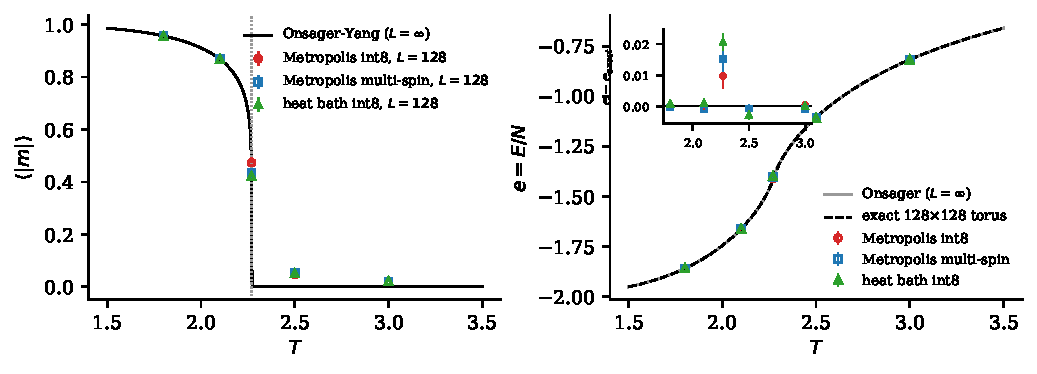
\includegraphics[width=\linewidth]{../figures/validation.pdf}
\caption{2D validation at $L=\valLtwo$. Left: $\langle|m|\rangle$ against the Onsager--Yang
spontaneous magnetisation. Right: energy per spin against Onsager's infinite-lattice result and
the exact energy of the finite torus; inset: deviation from the exact finite-lattice value.}
\label{fig:validation}
\end{figure}

\begin{figure}[t]
\centering
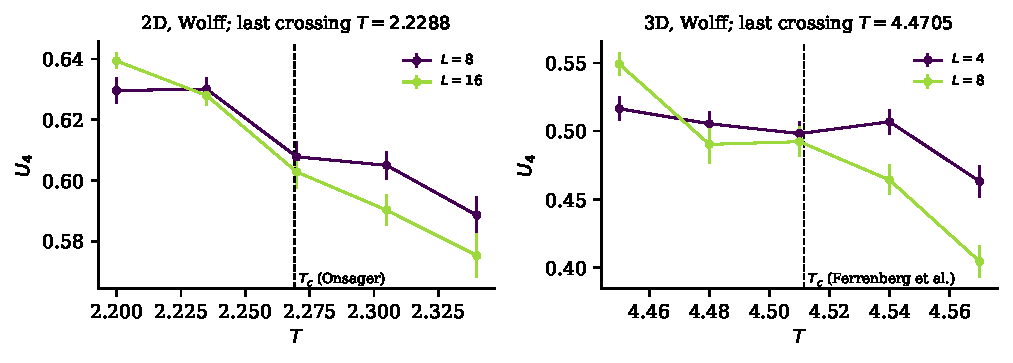
\includegraphics[width=\linewidth]{../figures/binder.pdf}
\caption{Binder cumulants from Wolff simulations; the dashed line is the exact (2D) or
reference (3D, \citealp{Ferrenberg2018}) critical temperature.}
\label{fig:binder}
\end{figure}

\paragraph{Bitwise identity.} With the same seed and start, \valIdentical{} of the
\valNIdentity{} backend/variant/algorithm/dimension combinations reproduce the NumPy oracle
bit for bit (\cref{tab:ladder}); the test suite checks this on every run.

\paragraph{Exact results.} \Cref{fig:validation} shows Metropolis (int8 and multi-spin) and
heat bath at $L=\valLtwo$. Against the exact finite-torus energy the largest deviation is
$\valEmaxErr$ and the largest deviation in units of the standard error is \valEmaxZ{}.
Below $T_c$, away from the critical region, $\langle|m|\rangle$ agrees with the infinite-lattice
Onsager--Yang result to $\valMmaxErr$.

\paragraph{Critical temperature.} The crossing of the two largest 2D Binder curves
(\cref{fig:binder}) is at $T=\valTcTwo$ (\valTcTwoErr\,\% from Onsager's $T_c$); in 3D at
$T=\valTcThree$ (\valTcThreeErr\,\% from $1/K_c$ of \citealp{Ferrenberg2018}), with the residual
shift expected from corrections to scaling at these sizes. 3D Metropolis and heat bath on the GPU
agree with 3D Wolff energies at $L=\valLthree$ within \valThreeZ{} standard errors.

\section{Performance}

\begin{figure}[t]
\centering
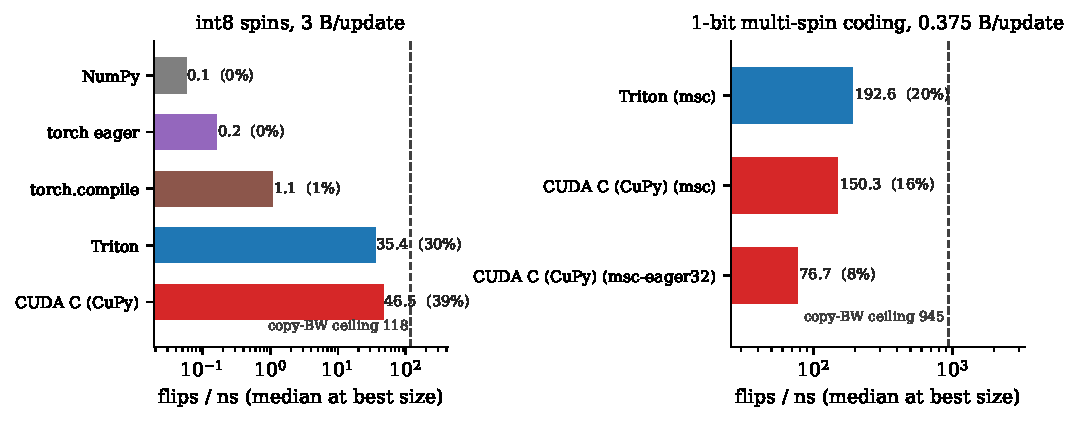
\includegraphics[width=\linewidth]{../figures/ladder.pdf}
\caption{Best throughput of each backend/variant (2D Metropolis at $T_c$, hot start); labels
give flips/ns and the percentage of the copy-bandwidth ceiling under the minimal traffic model.
Dashed: copy-bandwidth ceiling.}
\label{fig:ladder}
\end{figure}

\begin{figure}[t]
\centering
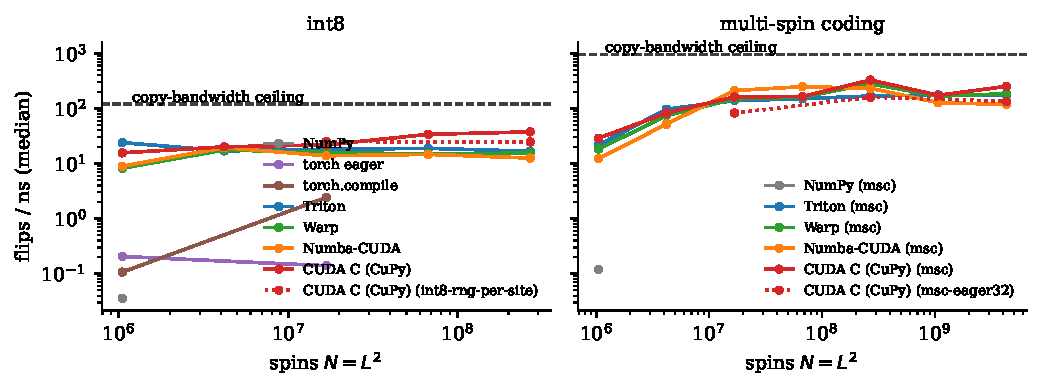
\includegraphics[width=\linewidth]{../figures/scaling.pdf}
\caption{Throughput against lattice size. Small lattices are bound by kernel-launch latency;
large lattices reach a plateau below the roofs of \cref{fig:roofline}. Dotted lines are the RNG ablations.}
\label{fig:scaling}
\end{figure}

\begin{figure}[t]
\centering
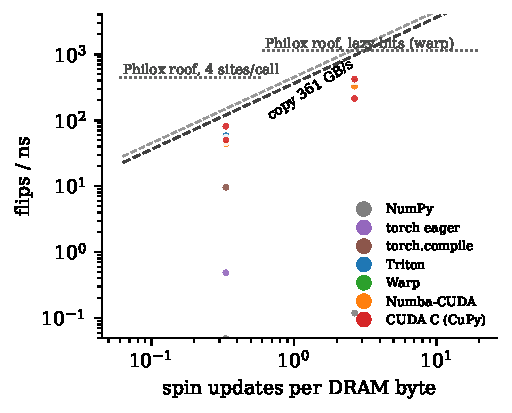
\includegraphics[width=0.6\linewidth]{../figures/roofline.pdf}
\caption{Roofline: throughput against spin updates per DRAM byte. Dashed: measured copy and
nominal bandwidth; dotted: Philox throughput divided by calls per update.}
\label{fig:roofline}
\end{figure}

\begin{table}[t]
\centering\small
\perfTable
\caption{Best median throughput per backend and variant (2D Metropolis at $T_c$) with effective
bandwidth under the minimal traffic model. Source: \texttt{results/\benchFile}.}
\label{tab:perf}
\end{table}

Measurements use \texttt{bench/run.py}: warm-up including JIT compilation, device
synchronisation around the timed region, at least \SI{0.5}{s} per timed run and the median of
five repeats. \Cref{fig:ladder,fig:scaling,tab:perf} summarise \nRuns{} runs on the
\gpuName{} (copy bandwidth \SI{\copyBW}{GB/s} measured, \SI{\specBW}{GB/s} nominal).

\paragraph{int8 rungs.} NumPy reaches \numpyFlips{} flips/ns. The tensor-op versions are
dominated by temporaries (PyTorch eager) or by the 64-bit emulation of Philox (\texttt{torch.compile}).
The best int8 kernel (\bestIntBackend) reaches \bestIntFlips{} flips/ns, \bestIntPctCopy\,\% of
the copy-bandwidth ceiling: int8 Metropolis is memory-bound, and the RNG is cheap once one Philox
call serves four sites (the per-site ablation runs at \ablPerSite{} flips/ns versus \ablCudaInt{}).

\paragraph{Multi-spin coding.} Packing cuts the traffic eightfold and raises the memory ceiling
to \memCeilMsc{} flips/ns, close to the per-warp Philox ceiling of \rngCeilMscWarp{} flips/ns.
Random numbers are the largest single cost: the eager ablation that always draws 32 bits per spin
reaches \ablEager{} flips/ns, the lazy kernel \ablLazy{} flips/ns. The best variant overall,
\bestBackend{} at $L=\bestL$, reaches \bestFlips{} flips/ns, \bestPctCopy\,\% of the copy
ceiling (\SI{\bestGBs}{GB/s} effective, \bestPctSpec\,\% of nominal) and \bestPctRngWarp\,\% of
the per-warp Philox ceiling, \speedupVsNumpy$\times$ the NumPy reference. Neither ceiling is
reached; we have not profiled which on-chip resource limits the packed kernels. The best kernel written entirely in a Python DSL, \bestPyBackend{}, reaches
\bestPyFlips{} flips/ns (\bestPyPctCopy\,\% of copy bandwidth).

\paragraph{3D.} The simple-cubic int8 kernels reach \bestThreeFlips{} flips/ns
(\bestThreeBackend, $L=\bestThreeL$, \bestThreePct\,\% of copy bandwidth).

\paragraph{Comparison with published codes.} \citet{Romero2020} report 420.8 flips/ns for their
optimised multi-spin code on a V100-SXM with HBM2 memory, about twice the nominal bandwidth of
our laptop part, using 4-bit spins and one 32-bit uniform per spin; \citet{Block2010} report
7.9 flips/ns on a Tesla C1060. Our best kernel reaches \bestFlips{} flips/ns, about the same
absolute rate on a part with half the nominal bandwidth. The gain is algorithmic (1 instead of
4 bits per spin, \bitsPerSpinWarp{} instead of 32 random bits per spin), not a property of the
host language, and it is a single-device statement on different hardware generations, not a
claim to exceed their throughput or their multi-GPU aggregates (but see
\cref{sec:headtohead}).

\subsection{Head-to-head with the reference CUDA implementation}
\label{sec:headtohead}

To compare on equal hardware we built and ran NVIDIA's reference code \citep{IsingGPURepo}
(commit \texttt{\cpCommit}) on our GPU. It contains five single-GPU programs for 2D
checkerboard Metropolis: a basic CUDA~C and a basic
Python version (Numba kernels, CuPy cuRAND uniforms), a tensor-core version and the optimised
4-bit multi-spin code of \citet{Romero2020}, and the current 1-bit code (\texttt{cuIsingModel})
of \citet{Bisson2025}, which draws its acceptance bits from a 16-entry lookup table (four
random bits per 32-bit draw). We compiled them with \texttt{nvcc} 13.4 for \texttt{sm\_86} and
did not change their sources or algorithms. The only patches are build flags: the target
architecture, C++17 for the CUB shipped with CUDA~13, and a force-included header that restores
two runtime-API overloads removed in CUDA~13 (for the tensor-core program it also provides the
half-to-double CUB sum used for the final magnetisation, outside the timed loop). The basic
Python script runs unchanged, with \texttt{cupy.cuda.curand} aliased to its current module.
\texttt{bench/counterparts.py} builds everything, runs both codes on the same lattices at
$T=T_c$, hot start, $J=1$, periodic boundaries, and records the commit and every patch in
\texttt{results/counterparts.json}.

Both codes report the same metric: $L^2$ times the number of sweeps divided by the time, where a
sweep updates both colours once. We parse the rate each program prints, so their timed regions
stay as written (host clock or CUDA events around the update loop; the basic codes include the
cuRAND call that fills one uniform per site). Each configuration runs once to size the sweep count, then
five times (median reported). As a check that both simulate the same model, the
energy per spin after \cpEnergySweeps{} sweeps from a hot start on $L=\cpEnergyL$ (\cpEnergySeeds{} seeds
each) is $\cpEnergyTheirs$ for \texttt{cuIsingModel} and $\cpEnergyOurs$ for our packed CUDA~C
kernel, within \cpEnergyMaxZ{} standard errors. The basic CUDA and basic Python programs share
the cuRAND stream and give \cpBasicIdentical{} magnetisations.

\ifthenelse{\equal{\cpProvisional}{true}}{\noindent\textbf{\textcolor{red!70!black}{Provisional:}}
the numbers in this subsection come from a short run on a shared GPU (mode
\texttt{\cpMode} of \texttt{bench/counterparts.py}); the final numbers come from its
\texttt{-{}-full} mode on an idle GPU.\par}{}

\begin{figure}[t]
\centering
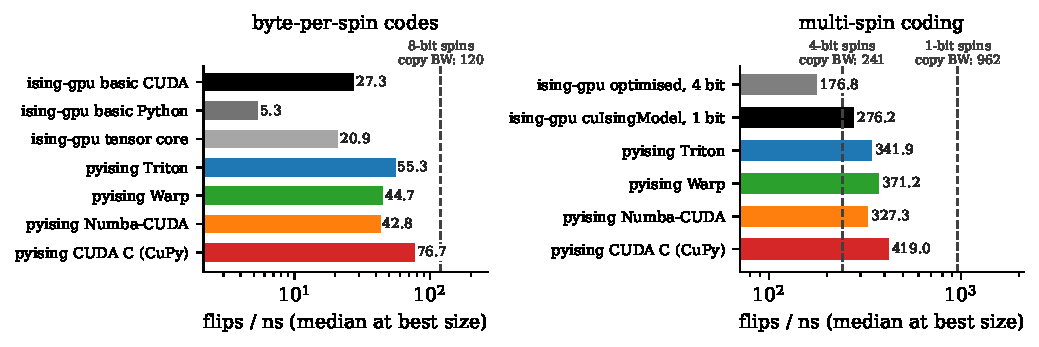
\includegraphics[width=\linewidth]{../figures/counterparts.pdf}
\caption{Same-GPU head-to-head, 2D Metropolis at $T_c$: best median over lattice sizes of
the NVIDIA/ising-gpu programs (black, grey) and of pyising (colours). Dashed: copy-bandwidth
ceilings for 8-, 4- and 1-bit spins under the minimal traffic model.}
\label{fig:counterparts}
\end{figure}


\paragraph{Byte-per-spin codes.} Basic CUDA~C reaches \cpRomeroBasicCudaFlips{}
flips/ns ($L=\cpRomeroBasicCudaL$); our best int8 kernel (\cpOursIntBackend) reaches
\cpOursIntFlips{} flips/ns, \cpRatioBasic$\times$ as much. Their program writes a 4-byte uniform per site to
DRAM and reads it back; ours draws random numbers inside the update kernel. The basic Python
program reaches \cpRomeroBasicPyFlips{} flips/ns; our best Python-DSL int8 kernel
(\cpOursPyIntBackend) reaches \cpOursPyIntFlips{} (\cpRatioPyBasic$\times$). Its Numba kernel
computes the acceptance probability in double precision (Python floats are 64-bit; checked in
the PTX), which a GeForce GPU executes at 1/64 of the FP32 rate (the V100 of the original paper:
1/2). The slowdown comes from FP64 arithmetic on a consumer GPU, not from Python itself. The
tensor-core program reaches \cpRomeroTensorFlips{} flips/ns.

\paragraph{Multi-spin codes.} The 4-bit code of \citet{Romero2020} reaches
\cpRomeroOldFlips{} flips/ns ($L=\cpRomeroOldL$, \cpPctCopyOld\,\% of copy bandwidth at
1.5\,B/update), and the 1-bit \texttt{cuIsingModel} reaches \cpRomeroOptFlips{} flips/ns
($L=\cpRomeroOptL$, \cpPctCopyOpt\,\% of copy bandwidth). On this GPU our best packed kernel
(\cpOursMscBackend, \cpOursMscFlips{} flips/ns at $L=\cpOursMscL$) is \cpOptCompare{} the 1-bit
reference (ratio \cpRatioOpt) and \cpOldCompare{} the 4-bit one (ratio \cpRatioOld). The best
kernel written in a Python DSL (\cpOursPyMscBackend, \cpOursPyMscFlips{} flips/ns) is
\cpPyOptCompare{} the 1-bit reference (ratio \cpRatioPyOpt). None of the packed codes reaches its
memory ceiling, so the difference lies in the work per spin. The 4-bit code moves four times
the bytes and draws one 32-bit uniform per spin. \texttt{cuIsingModel}
draws two 4-bit table lookups per four spins (16 random bits per spin) at every temperature.
Our lazy comparison draws \bitsPerSpinWarp{} bits per spin, counted at the slowest thread of
each warp at $T_c$. \texttt{cuIsingModel} also synchronises with the host after every
half-sweep, which costs most on small lattices. We have not profiled their kernels on this GPU and do not
attribute the whole gap to the random numbers; their kernel parameters were tuned on
other GPUs, so the ranking holds for this laptop GPU only and says nothing about their
multi-GPU results.

\section{Discussion}

\paragraph{What carries the speed.} Three choices matter more than the language: a layout that
touches only active spins, one random draw per spin amortised over many spins (four sites per
Philox call for int8; 64 lanes per random word for packed spins), and a lazy comparison that
spends random bits only on undecided lanes. Once these are in place, kernels written in Python reach
\dslIntPctCuda\,\% (int8, \dslIntBackend) and \dslMscPctCuda\,\% (packed, \dslMscBackend) of the
throughput of the NVRTC-compiled CUDA~C reference; none of them overtakes it.

\paragraph{Threats to validity.} (i) A single laptop GPU: clocks and power limits throttle under
sustained load, and the copy ceiling itself varies by a few percent between runs; we report
medians with min/max. (ii) During development the GPU was shared; every number reported here comes
from one serial run on an idle GPU. (iii) The CUDA~C reference is compiled by NVRTC with
\texttt{-use\_fast\_math}, not by \texttt{nvcc} with tuned flags; a different compiler could
change the reference by some percent. (iv) The lazy kernel's cost depends on temperature (fewer
undecided lanes deep in the ordered phase); we benchmark at $T_c$. (v) The packed variant is
implemented for 2D Metropolis only; heat bath and 3D use int8 spins.

\section{Conclusion}
A single Python package drives seven backends of the same algorithm with bit-identical results
and validated physics. On a laptop GPU, Python-hosted multi-spin-coding kernels reach
\bestFlips{} spin flips per ns (\bestPctCopy\,\% of the memory roofline; \bestPyFlips{} for a
kernel written entirely in a Python DSL) by spending effort where the roofline says it matters: bytes per update and random bits per spin.

\section*{Code availability}
Code, benchmark JSON, figure scripts and this paper: \url{https://github.com/walidhemati/pyising}
(MIT licence). \texttt{bench/run.py -{}-full}, \texttt{bench/counterparts.py -{}-full},
\texttt{figures/make\_figures.py} and \texttt{tectonic paper/paper.tex} regenerate every number
and figure.

\setlength{\bibsep}{2pt plus 1pt}
\bibliographystyle{unsrtnat}
\bibliography{references}

\end{document}
